\documentclass{article}

\usepackage[letterpaper,top=3cm,bottom=2cm,left=3cm,right=3cm,marginparwidth=1.75cm]{geometry}

\usepackage{amsmath}
\usepackage{amssymb}
\usepackage{graphicx}
\usepackage{float}
\usepackage{algpseudocode}

\title{CPSC 322 Introduction to AI}
\author{Kaitian Xie}
\date{May 11, 2019}

\graphicspath{ {./images/} }

\begin{document}

\maketitle
\pagebreak

\section{Introduction}

\section{Search}

\subsection{Intro to Search}
% TODO

\subsubsection{Directed Acyclic Graph (DAG)}

\begin{itemize}
    \item \textbf{Directed ayclic graph}: a graph with no cycles and where the arcs have associated directions.
\end{itemize}

\subsubsection{Search with Costs}

\begin{itemize}
    \item \textbf{Cost of a path}: sum of costs of its arcs $cost(<n_0, \ldots, n_k>) = \sum\limits_{i=1}^{k} (<n_{i-1}, n_i>)$
    \item \textbf{Optimal solution}: solution with minimal cost.
\end{itemize}

\subsubsection{Heuristic}

\begin{itemize}
    \item \textbf{Search heuristic ($h(n)$)}: an estimate of the cost of the lowest-cost path from node $n$ to a goal node.
    \item \textbf{Admissible heuristic}: $h(n)$ is admissible if it is never an overestimate, i.e. $h(n)$ is a lower bound. To construct an admissible heuristic, we can either:
    \begin{itemize}
        \item drop some constraints or
        \item make less restrictions on actions
    \end{itemize}
    \item \textbf{Dominance}: If $h_2(n) \geq h_1(n)$ for every state $n$ (both admissible), then $h_2$ dominates $h_1$.
    \item we can combine two admissible heuristic functions: $h(n) = max\{h_1(n), h_2(n)\}$.
\end{itemize}

\subsubsection{Uninformed Search vs Heuristic Search}

\begin{itemize}
    \item \textbf{Uninformed}: not taking the goal into account until the goal state is reached.
    \item \textbf{Heuristic}: there exists extra knowledge to guide the search.
\end{itemize}

\subsection{Generic Search Algorithm}

\begin{algorithmic}
    \Require{a graph, a start node $n_0$, $goal(n)$}
    \State{$frontier := [<n_0>]$}
    \While{$frontier$ is not empty}
        \State{Select and remove a path $<n_0, \ldots, n_k>$ from $frontier$}
        \If{$goal(n_k)$}
            \State{return $<n_0, \ldots, n_k>$}
        \EndIf
        \For{every neighbor $n$ of $n_k$}
            \State{Add $<n_0, \ldots, n_k, n>$ to $frontier$}
        \EndFor
    \EndWhile
\end{algorithmic}

\begin{figure}[H]
    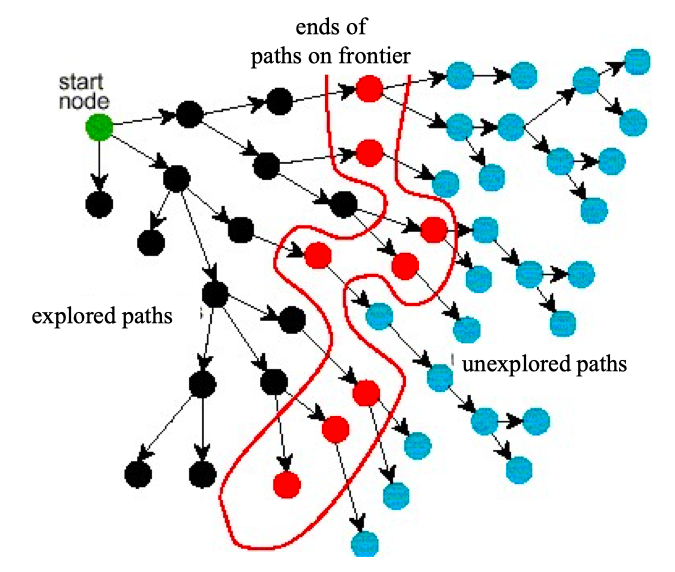
\includegraphics[width=\textwidth]{generic_search_algo_visualization}
    \centering
\end{figure}

\subsubsection{Branching Factor ($b$)}

\begin{itemize}
    \item \textbf{Forward branching factor}: number of arcs going out of a node
    \item \textbf{Backward branching factor}: number of arcs going into a node
\end{itemize}

\subsubsection{Complete \& Optimal}

\begin{itemize}
    \item \textbf{Complete}: can find a solution.
    \item \textbf{Optimal}: can find the best solution.
\end{itemize}

\subsubsection{Complexity}

\begin{itemize}
    \item \textbf{Time complexity}: amount of time needed in the worst-case scenario; expressed in terms of maximum path length ($m$) and maximum branching factor ($b$).
    \item \textbf{Space complexity}: amount of space needed in the worst-case scenario; expressed in terms of $m$ \& $b$.
\end{itemize}

\subsection{Depth-First Search (DFS)}

\begin{itemize}
    \item $frontier$ is a stack $[p_1, p_2, \ldots, p_k]$
    \item neighbors of last node of $p_1$ are $\{n_1, \ldots, n_k\}$
    \item
    \begin{algorithmic}
        \While{$frontier$ is not empty}
            \State{$p := frontier.pop()$}
            \State{$n_{end} := $ last node of $p$}
            \If{$goal(n_{end})$}
                \State{Return $p$}
            \EndIf
            \State{$frontier.push((p, n_1), \ldots, (p, n_k))$}
        \EndWhile
    \end{algorithmic}
    \item not complete because DFS may get ``stuck'' in a graph that has cycles.
    \item not optimal because DFS may return a longer solution while a shorter solution exists
    \item time complexity: $O(b^m)$
    \item space complexity: $O(bm)$
    \item DFS is appropriate when:
        \begin{itemize}
            \item space is restricted.
            \item there are many solutions, perhaps with long path solutions, particularly for the case in which all paths lead to a solution.
        \end{itemize}
    \item DFS is inappropriate when:
        \begin{itemize}
            \item cycles
            \item shallow solution
            \item optimality is needed
        \end{itemize}
\end{itemize}

\subsection{Breadth-First Search}

\begin{itemize}
    \item $frontier$ is a queue $[p_1, p_2, \ldots, p_k]$
    \item neighbors of last node of $p_1$ are $\{n_1, \ldots, n_k\}$.
    \item
    \begin{algorithmic}
        \While{$frontier$ is not empty}
            \State{$p := frontier.poll()$}
            \State{$n_{end} := $ last node of $p$}
            \If{$goal(n_{end})$}
                \State{Return $p$}
            \EndIf
            \State{$frontier.offer((p, n_1), \ldots, (p, n_k))$}
        \EndWhile
    \end{algorithmic}
    \item complete because it doesn't get stuck in cycles
    \item optimal because it guarantees to find the path that involves the fewest paths
    \item time complexity: $O(b^m)$
    \item space complexity: $O(b^m)$
\end{itemize}

\subsection{Iterative Deepening Search}

\begin{itemize}
    \item
        \begin{itemize}
            \item Look with DFS for solution at depths $1, 2, \ldots$
            \item If a solution can't be found at depth $D$, try again at depth $D+1$
            \item depth-bounded depth-first searcher
            \item given a bound $B$, assume the paths of length $B$ can't be expanded.
        \end{itemize}
    \item time complexity: $O(b^m)$

    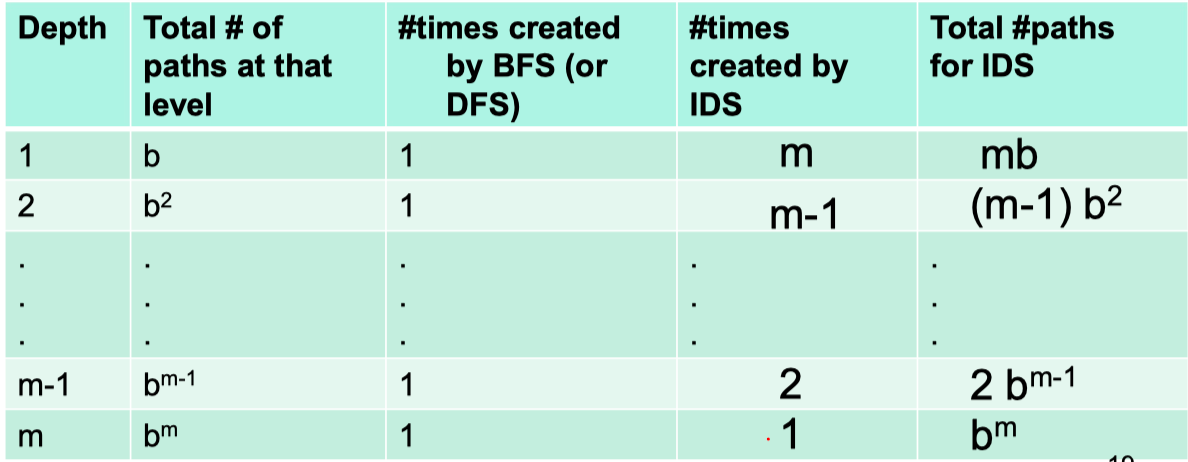
\includegraphics[scale=0.3]{ids_time_complexity}
    
    \begin{align*}
        b^m  + 2b^{m-1} + 3b^{m-2} + \ldots + mb 
        &= b^m (1 + 2b^{-1} + 3b^{-2} + \ldots + mb^{1-m}) \\
        & \leq b^m \sum\limits_{i=1}^{\infty} ib^{1-i} \\
        &= b^m (\frac{b}{b-1})^2 \\
        &= O(b^m)
    \end{align*}
\end{itemize}

\subsection{Lowest-Cost-First Search (LCFS)}

\begin{itemize}
    \item
    \begin{itemize}
        \item Select a path with the lowest cost from $frontier$ (a priority queue).
        \item not complete if there exists a cycle with zero or negative arc costs, otherwise it is complete
        \item not optimal if negative costs exist, otherwise it is optimal
        \item time complexity: $O(b^m)$
        \item space complexity: $O(b^m)$
            \begin{itemize}
                \item costs are equal $\Rightarrow$ BFS
            \end{itemize}
    \end{itemize}
\end{itemize}

\subsection{Best-First Search}

\begin{itemize}
    \item Select a path from the $frontier$ with minimal h-value (for the end node).
    \item The $frontier$ is implemented by a priority queue order by h-value.
    \item This is a greedy approach since it always takes a locally best path.
    \item not complete: if there exist low h-values in a cycle, BestFS gets stuck.
    \item not optimal: a heuristic might be misleading.
    \item time complexity: $O(b^m)$
    \item space complexity: $O(b^m)$
    \item BestFS is appropriate when:
        \begin{itemize}
            \item $h(n)$ is very good.
        \end{itemize}
\end{itemize}

\subsection{$A^{*}$}

\begin{itemize}
    \item LCFS + BestFS
    \item $f(p) = cost(p) + h(p)$
    \item The $frontier$ is implemented by a priority queue ordered by f-value.
    \item $A^{*}$ always selects a path that has the lowest estimated total distance to a goal.
    \item complete: $a^{*}$ always tests shorter underestimate of the total cost, so not missing anything
    \item optimal: $A^{*}$ is optimal if:
        \begin{itemize}
            \item $b$ is finite
            \item costs are strictly positive
            \item $h(n)$ is non-negative and admissible
        \end{itemize}
    \item proof of optimality: \textit{Lecture 8 slides 24-32}
    \item optimal efficiency: among all optimal algorithms that start from the same start node and use the same heuristic, $A^{*}$ expands the minimal number of paths.
\end{itemize}

\subsection{Branch-and-Bound Search (B\&B)}

\begin{itemize}
    \item $frontier$ implemented a stack, similar to DFS
    \item order of adding neighbours can be customized
    \item keeps track of a lower bound and an upper bound on a each path:
        \begin{itemize}
            \item lower bound: $LB(p) = f(p) = cost(p) + h(p)$
            \item upper bound: $UB = \text{cost of the best solution found so far}$ (initialize $UB = \infty$)
        \end{itemize}
    \item when a path $p$ is selected for expansion
        \begin{itemize}
            \item if $LB \geq UB$: remove $p$ from $frontier$
            \item else expand $p$
        \end{itemize}
    \item not complete: B\&B gets stuck in a graph with cycles
    \item optimal, but not optimal efficient
    \item time complexity: $O(b^m)$
    \item space complexity: $O(mb)$ (like DFS)
\end{itemize}

\subsection{Iterative Deepening $A^{*}$ ($IDA^{*}$)}

\begin{itemize}
    \item search depth-first, but to a fixed depth/bound
    \item depth measured in f-values
    \item if you don't find a solution, update the bound with the lowest f-value that passed the previous bound
    \item time complexity: $O(b^m)$
    \item space complexity: $O(mb)$
\end{itemize}

\subsection{Memory-Bounded $A^{*}$ ($MBA^{*}$)}

\begin{itemize}
    \item keep $frontier$ in memory as we can
    \item if we need to free some memory, we delete:
        \begin{itemize}
            \item the worst paths (with highest f-values)
            \item ``back them up'' to a common ancestor
            \item update $h(n)$ of the ancestor if possible
        \end{itemize}
\end{itemize}

\subsection{Summary of Search Strategies}

\begin{figure}[H]
    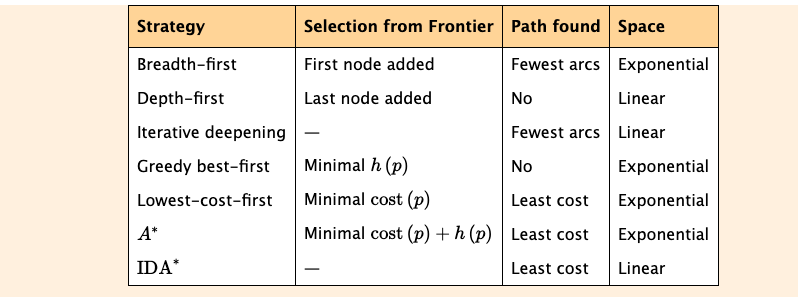
\includegraphics[width=\textwidth]{summary_of_search_strategies}
    \centering
\end{figure}

\subsection{Cycle Checking}

\begin{itemize}
    \item Prune a path that ends in a node already on the path
    \item Pruning doesn't remove an optimal solution.
    \item linear time complexity
\end{itemize}

\subsection{Multiple-Path Pruning}

\begin{itemize}
    \item Prune a path to node $n$ that you already found a path to.
\end{itemize}

\end{document}
